\documentclass[a4paper]{article}
\usepackage{listings}
\usepackage{graphicx}
%\usepackage[scale=.7]{geometry}
\usepackage{amsmath}
\usepackage{float}
\usepackage{acronym}
\usepackage{cite}
\usepackage{url}
\usepackage[usenames, pdftex]{color}

\acrodef{WSM}[WSM]{Weighted Scan Matching}
\acrodef{ICP}[ICP]{Iterated Closest Point}
\acrodef{RANSAC}[RANSAC]{Random Sample Consensus}
\acrodef{PFH}[PFH]{Point Feature Histograms}
\acrodef{FPFH}[FPFH]{Fast Point Feature Histograms}
\acrodef{SLAM}[SLAM]{Simultaneous Localization and Mapping}
\acrodef{PCL}[PCL]{Point Cloud Library}
\acrodef{SAC-IA}[SAC-IA]{SAmple Consensus Initial Alignment}

\title{Registration using a RGB-D camera\\
{\large Project A.I. / Individual project}}

\author{Carsten van Weelden \\ 0518824 \\ \texttt{cvanweelden@gmail.com} \and Thomas van den Berg \\ 5789346 \\ \texttt{Thomas.G.vandenBerg@gmail.nl} \and
 \small{Supervisor:} \\ Arnoud Visser \\ University of Amsterdam\\
  The Netherlands}

\date{\today}




\begin{document}
\maketitle

\section{Introduction}

In this project we familiarized ourselves with methods for 3D registration of images captured with cheap RGB-D sensors such as the Kinect. A Kinect mounted on a moving robot could replace both it's RGB camera and it's range finder. Another application would be affordable 3D reconstructions of the insides of buildings. For these applications we need to \emph{register} consecutive frames to the same global coordinate space. In effect, we need to find the transformation that the camera made in between the captured frames. The robot's odometry can sometimes be used to get an initial estimate of the transformation, but in a scenario where the RGB-D camera is hand-held this is not possible. For this reason we focused on the registration step only. 

The combined RGB and depth data forms a \emph{point cloud}: a set of 3D coordinate points indicating where the sensor measured a solid object. Assuming that there is enough overlap between each pair of consecutive point clouds, we find a good registration by finding an optimal way to fit the two clouds. We've experimented with different registration methods, and we'll report on their performance and whether it degrades under certain circumstances.

\section{Background}

\subsection{Registration}

\subsubsection{ICP Based Registration}

A basic method used in almost every approach to 3D registration is \ac{ICP}\cite{besl1992method}, it is an expectation maximization method that iteratively minimizes the distance between each point and it's closest neighbor. Though \ac{ICP} is currently used mostly as a refinement step for more advanced algorithms, there are still some papers describing experiments where using \ac{ICP} as the main registration procedure has been successful [[WHICH]]. 

In \cite{segal2009generalized}, an extension to \ac{ICP} was introduced that takes into account the local characteristics of the matched points. This Generalized-ICP gives a higher weight to point correspondence errors if they are in a direction perpendicular to the estimated plane. It is mentioned in both \cite{rusinkiewicz2001efficient} and \cite{segal2009generalized} that using this extension prevents the application of a closed-form solution to the minimization step.

\ac{WSM} removes a simplyfying assumption from \ac{ICP}, namely that ``the range scans of different poses sample the environment's boundary at \emph{exactly} the same points''~\cite{pfister2002weighted}. In range scans, it often occurs that the points are much further apart in some areas of the model, because of the angle of the local surface or the distance from the sensor. The point-to-point error in these areas could easily be much greater, this is what the authors take into account by introducing an error which they name the \emph{correspondence error}. They model the variance of this error based on the distances to the closest model points, \cite{slamet2008boosting} give a clear illustration in their Figure 1. 

In a sense, Generalized-ICP and \ac{WSM} are similar in that they make an explicit model of the error that the minimization step aims to minimize, based on the local characteristics. This has some clear advantages in terms of accuracy, but the extra computational costs are significant.

\subsubsection{Feature Based Registration}

An alternative to \ac{ICP} based registration is feature-based registration in which the transformation between frames is estimated from correspondences between feature points in 3D space, usually combined with \ac{RANSAC}. In stead of matching each point in the cloud to it's closest neighbour, characteristic points are extracted, and a feature \emph{descriptor} is calculated for each. Based on these descriptors, the feature points are matched to their counterparts in the other frame to get a number of \emph{correspondences}. Not all these correspondences may be correct though, so \ac{RANSAC} is often used to filter the outliers. 

\cite{rusu2009fast} describes such an approach. In it, \ac{PFH} are used as feature descriptors. For each point, these features are based on the properties of points in its neighborhood. To elaborate, every pair of points within the neighborhood (Figure~\ref{fig:fpfh}) generates a number of features based on their angle with respect to the local normal. Because the number of neighbors can vary, a histogram is created. Initially, every single point is used to generate a descriptor. Then, to speed up the matching and make it more robust, only \emph{unique} feature points are selected, i.e. points whose descriptors are different from the mean descriptor. \ac{RANSAC} is then used to find the best feature point correspondences.  

\begin{figure}[htbp]
    \centering
        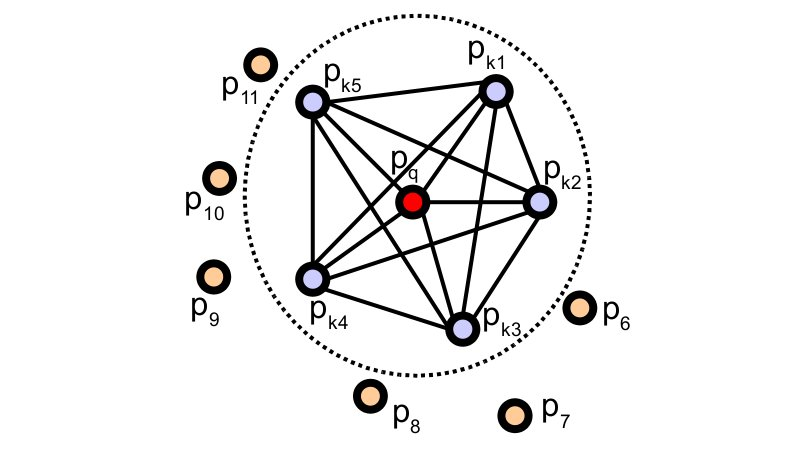
\includegraphics[height=4cm]{ims/fpfh.jpg}
    \caption{The PFH dependency diagram (image from \cite{rusu2009fast}). It indicates that every pair of points in the neighborhood generates features.}
    \label{fig:fpfh}
\end{figure}

\subsection{Applications}

\subsubsection{Global registration}

Global registration is the problem of reconstructing a global model from a sequence of frames. Each frame has to be registered to a global coordinate system, generally defined by the axes of the first frame of the sequence. One challenge in applying registration algorithms to this problem is that errors in pairwise registration accumulate over time. Other challenges associated with global registration are integrating the registered noisy measurements into a smooth global model and dealing with dynamic scenes in which objects move between frames.

In the KinectFusion project presented in \cite{izadi2011kinectfusion,newcombe2011kinectfusion} \ac{ICP} is used to register depth frames captured using a Kinect camera to build a global model. For the model they use the volumetric representation described in \cite{curless1996volumetric}. 
%Explain how this deals with registration noise and error build up.

\subsubsection{\ac{SLAM}}

%This is also know as \emph{visual odometry} and a more complete overview can be found in \cite{scaramuzzavisual,fraundorfervisual}. 

As mentioned before, the registration step that we focus on in this report provides us with all the information needed to perform \ac{SLAM} using \emph{visual odometry}. Visual odometry is the converse problem to registration: by finding the relative transformation between frames we can also compute the egomotion of the camera. In \ac{SLAM} we use this registration step for localization, and by merging the registered 3D images we create a map of the environment. However, though the registration step is essential, it is far from sufficient for good localization. The most notable problem is the \emph{error buildup}; cumulative errors in the registration steps cause an ever greater error in the final position estimation. This can lead to a defective \emph{loop closing}: when the sensor comes to a place it has been before, the built-up error will almost surely cause this to be registered as a different position from the original one. If this loop can be detected at all, it is still necessary to re-register all earlier frames so that the loop is closed. 
%In \cite{pfingsthorn2008scalable} \ac{WSM} is combined with loop closing and a manifold data structure?

In \cite{slamet2008boosting} \ac{ICP} and \ac{WSM} are applied to solve the \ac{SLAM} problem in 2D, but instead of registering each frame to the previous frame they store all registered frames in a quad tree and register the frames against multiple previously registered frames. They show that this leads to better results than incremental pair-wise registration of frames.

In \cite{nuchter20076d} \ac{ICP} is used on point cloud data to solve the \ac{SLAM} problem in 3D. They use a cached version of the kd-tree data structure to make this feasible in real-time. They state that in combination with loop closing and model refinement this leads to accurate results.

\section{Experiments}

We ran a number of experiments to find out about the behavior of different registration methods and their performance in different settings. One of the most influential properties of the input data is the magnitude of the transformation between frames. To clarify; a slow-driving robot will record frames that are are mostly similar, making it easier to find corresponding points or features in both frames, whereas a shaky handheld RGB-D camera might output frames with a much larger discrepancy. Typically, a set of frames with small transformations between them is an easier input to a registration algorithm. However, when building a global model or using the registration to perform SLAM, each step contributes an amount of error to the final results, therefore it is better to use as few frames as possible as long as the registration still works reasonably well. [[Is er een artikel waar ze frames overslaan onder bepaalde condities?: dat even citeren.]]

Our first experiment examines whether the total buildup of error is larger when using more frames, we did this by [[...]] We've also run the registration on the dataset to create a global model, to show that the buildup of error can be quite catastrophic for this purpose.

The rest of our experiments focus on the advantages of using feature-based registration methods when the magnitude of the relative transform between frames gets larger. All of these experiments consist of registering each frame $i$ to the $i-n^{\mathrm{th}}$ frame, with $n = 1,2,3,...$. By skipping frames in this manner, we artificially create a larger transformation for the registration step to solve. We expect to see that the feature-based methods are better at dealing with this larger transformation.

\subsection{Datasets}

We use two RGB-D datasets from the benchmark presented in \cite{sturm11rss-rgbd}. In addition to the RGB-D data, it contains a ground truth for the camera's position obtained using a motion capture system which we use for evaluation. Both datasets are captured as an indoor scene around a desk with several objects on it.

The specific datasets that we use are \texttt{freiburg2\_xyz} and \texttt{freiburg1\_desk}\footnote{Available at \url{http://cvpr.in.tum.de/data/datasets/rgbd-dataset}}. The \texttt{xyz} dataset was recorded with a slow and steady movement of the RGB-D sensor, so that the magnitude of the translation is constant. Rotation is kept to a minimum. The \texttt{desk} dataset is recorded with much faster movement, leading to larger differences between subsequent frames as well as motion blur and rolling shutter effects. It contains both translation and rotation between frames.

\subsection{Implementation}

For our implementation we use \ac{PCL} \cite{Rusu_ICRA2011_PCL}. We use the standard \ac{ICP} implementation provided by this library with a maximum of 25 iterations and maximum correspondence distance of 0.25m. We refer to this method in our figures as \texttt{ICP}.

 For our feature based method we use the implementation of the \ac{SAC-IA} method from \cite{rusu2009fast} as implemented for this library, limited to 1000 iterations with a maximum correspondence distance of 0.1m and minimum distance of 0.5m between the samples used for the \ac{RANSAC} method. For the \ac{FPFH} features we use a radius of 0.1m for normal estimation and 0.5m for feature computation. This implementation does not apply the Levenberg-Marquardt algorithm as described in \cite{rusu2009fast}. In stead, we test this method without refinement after the feature-based alignment and with the ICP-based refinement. We refer to these methods as \texttt{FPFH} and \texttt{FPFH+ICP} respectively.
 
 In all cases we remove sparse outliers by removing all points whose mean distance to its 50 nearest neighbors is more than one standard deviation from the overall mean and we subsample by taking one point for each 5cm$^3$ voxel.


\subsection{Results}

Using \ac{FPFH} with \ac{ICP} we registered frames from the two datasets as well as from two datasets that we recorded ourselves. This section presents some of the qualitative results before we evaluate against the benchmark ground truth in the following sections.

Figure \ref{fig:xyz_results} shows the result of registering the first [[how many?]] frames of the \texttt{xyz} dataset. We can clearly see the effect of errors in the pairwise registration where, after a single mis-estimation of the transformation between frames, all following frames are also badly registered, resulting in duplicate objects such as the teddy bear behind the desk and the calibration pattern to the right.

\begin{figure}[htbp]
    \centering
        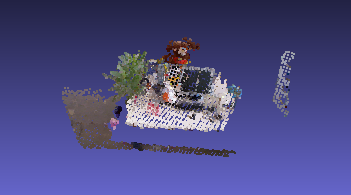
\includegraphics[width=\textwidth]{ims/xyz_results.png}
    \caption{Registration results on the \texttt{xyz} dataset.}
    \label{fig:xyz_results}
\end{figure}

\subsection{Accumulated error over time}
\label{accumulated_error}

The registration step registers a pair of frames with a certain error (which we investigate in section \ref{registration_error}. For global registration and \ac{SLAM} this error accumulates as frames are sequentially registered to previously registered frames. One way to deal with this problem is by skipping frames. Registering fewer frames means accumulating less error, but the overlap between each pair of frames needs to be large enough for successful registration. 

We investigate the effect of skipping frames by looking at the registration error after a fixed duration with varying offsets between registered frames. We calculate the mean error over 50 segments of 1 second starting at frame 1 to 50 for the \texttt{freiburg2\_xyz} and \texttt{freiburg1\_desk} datasets.

\subsubsection{Results}

Figure \ref{fig:accumulated_rotation_error} shows the error in orientation after registering frames over 1 second for both datasets. The left graph shows the \texttt{freiburg2\_xyz} and clearly shows the error decreasing for the \ac{FPFH} method, although when using \ac{ICP} the effect is less noticeable. All the methods perform well with high frameskip since the movement in this dataset is small enough such that frames have considerable overlap even if the duration between the frames being captured was large.

With the \texttt{freiburg1\_desk} dataset (graph on the right) we see that increasing the number of frames skipped reduces the accumulated error for the feature-based methods up to a point where the error starts to increase over the base level for registering all frame pairs. Overlap between frames in this dataset is much smaller because of the faster movement of the camera. The frames are harder to register and we see a tradeoff between limiting the amount of error accumulated over consecutive transformations and the error in the registrations themselves. Compared to \ac{ICP} the feature-based methods are better able to handle large transformations and thus have a more favorable balance between these two sources of error.

\begin{figure}[htbp]
    \centering
        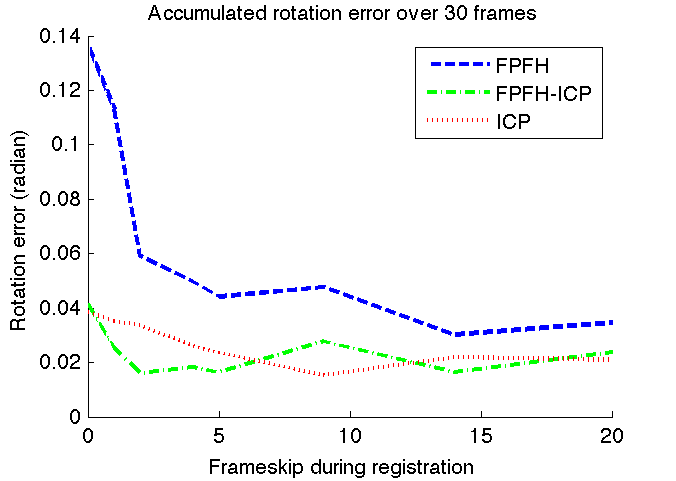
\includegraphics[width=0.49\textwidth]{ims/xyzAccumulatedrotationerrorover30frames.png}
        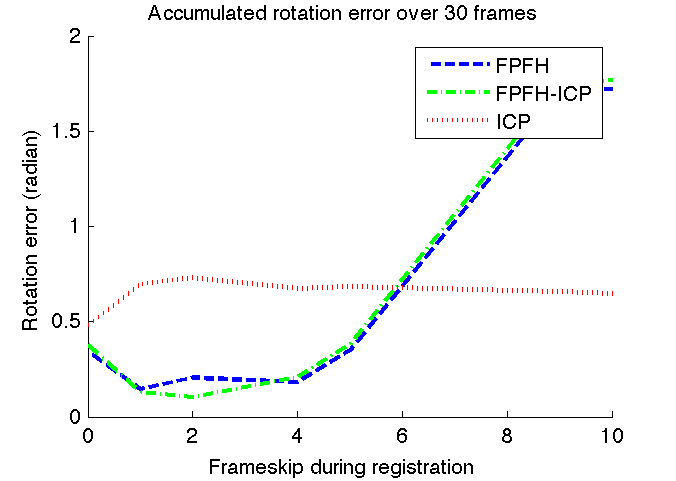
\includegraphics[width=0.49\textwidth]{ims/deskAccumulatedrotationerrorover30frames.png}
    \caption{Rotation error after registering 30 consecutive frames (1 second) for the  \texttt{freiburg2\_xyz} dataset on the left and the \texttt{freiburg1\_desk} on the right.}
    \label{fig:accumulated_rotation_error}
\end{figure}

Figure \ref{fig:accumulated_translation_error} shows the translation error after registration for the same runs. The results show the same behavior as the results for the translation error. 

\begin{figure}[htbp]
    \centering
        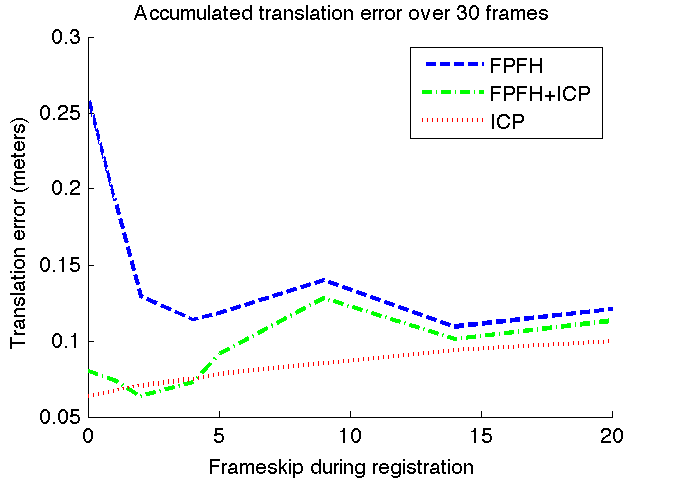
\includegraphics[width=0.49\textwidth]{ims/xyzAccumulatedtranslationerrorover30frames.png}
        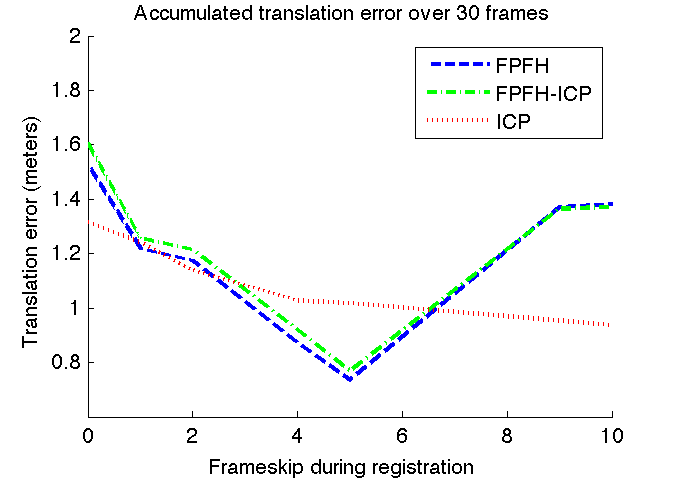
\includegraphics[width=0.49\textwidth]{ims/deskAccumulatedtranslationerrorover30frames.png}
    \caption{Translation error after registering 30 consecutive frames (1 second) for the  \texttt{freiburg2\_xyz} dataset on the left and the \texttt{freiburg1\_desk} on the right.}
    \label{fig:accumulated_translation_error}
\end{figure}

These results show that the optimal value for the offset between registered frames is dependent on the dataset, specifically on how large the transformations between poses are, and how well the method can handle frame pairs with small overlap.

\subsection{Registration error}
\label{registration_error}

We show how the error for registering a frame pair increases as the frames are farther apart by computing the rotation and translation error for frame pairs with varying offsets between frames. Here we use the frame offset as a proxy for the magnitude of the transformation, but we also show how the rotation and translation magnitudes vary with the frame offset.

We calculate the rotation error as the angular distance between the true rotation $q$ and the estimated rotation $\hat q$ which we calculate as $min(\theta, 2\pi - \theta)$ where $\theta$ is the angle between the two rotations represented as quaternions: $\theta = 2 * cos^{-1}(q \cdot \hat q)$. %Dit hierboven heb ik opgeschreven omdat het nergens te vinden was.
The translation error is given as the euclidean norm of the difference between the true and estimated translation. We compute the mean errors over 50 frame pairs for up to 2 seconds apart from the start of the \texttt{freiburg2\_xyz} and \texttt{freiburg1\_desk} datasets.

\subsubsection{Results}


%\section{Results}

[[Laten zien dat de error buildup ervoor zorgt dat een globaal model een zootje wordt, op onze eigen dataset]]

\begin{figure}[H]
    \centering
        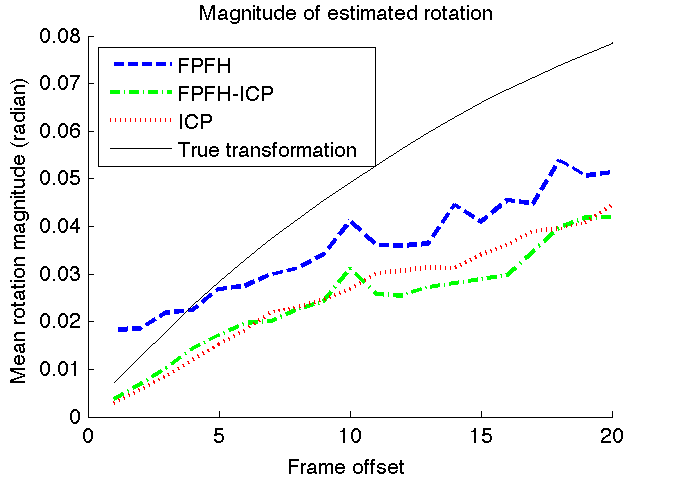
\includegraphics[width=0.49\textwidth]{ims/xyzMagnitudeofestimatedrotation.png}
        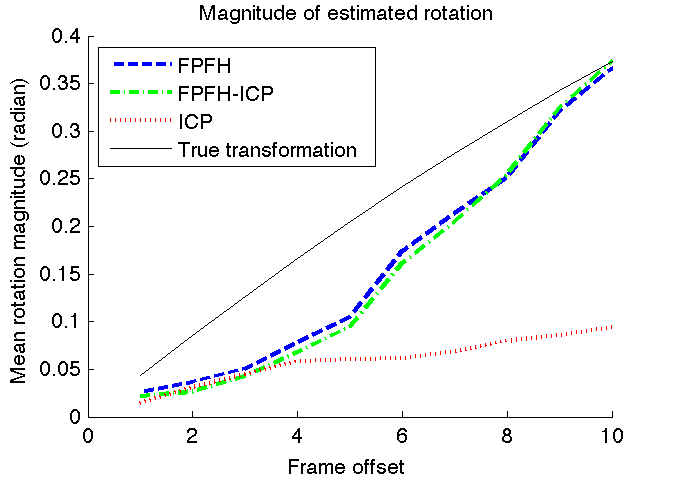
\includegraphics[width=0.49\textwidth]{ims/deskMagnitudeofestimatedrotation.png}
    \caption{The magnitude of the rotations estimated by the different methods on the two datasets, with \texttt{freiburg2\_xyz} on the left and \texttt{freiburg1\_desk} on the right. The x-axis represents the amount of frames between each registered pair.}
    \label{fig:rotation_magnitude}
\end{figure}

As can be seen in Figures~\ref{fig:rotation_magnitude} and~\ref{fig:translation_magnitude}, ICP tends to estimate a smaller transformation between frames, this can be explained by the fact that ICP is likely to move to the closest local minimum. Examining the results more closely, we see that when \ac{ICP} is preceded by an initial alignment step, the results are different, this indicates that \ac{ICP} finds a \emph{different} local minimum in those cases, albeit not always a better one.

\begin{figure}[H]
    \centering
        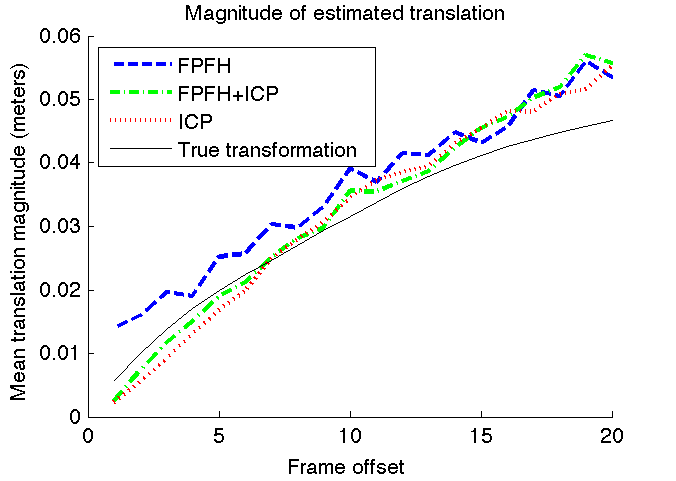
\includegraphics[width=0.49\textwidth]{ims/xyzMagnitudeofestimatedtranslation.png}
        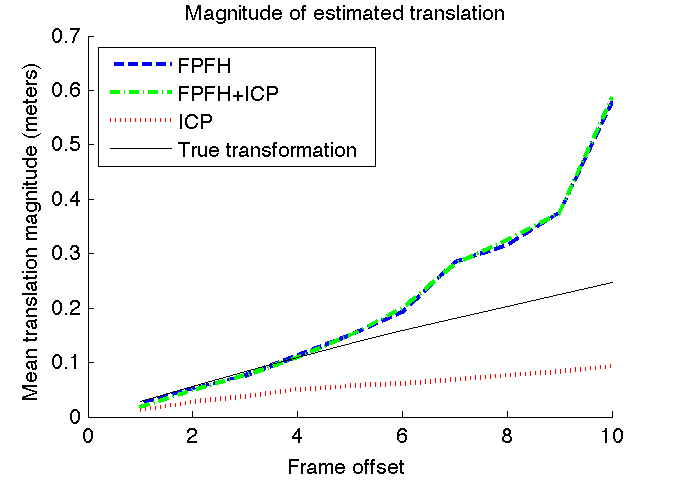
\includegraphics[width=0.49\textwidth]{ims/deskMagnitudeofestimatedtranslation.png}
    \caption{The magnitude of the translations estimated, like Figure~\ref{fig:rotation_magnitude}. }
    \label{fig:translation_magnitude}
\end{figure}


\begin{figure}[H]
    \centering
        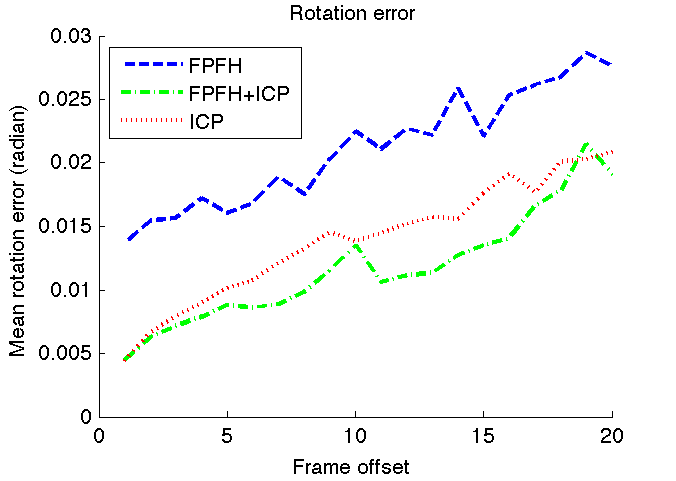
\includegraphics[width=0.49\textwidth]{ims/xyzRotationerror.png}
        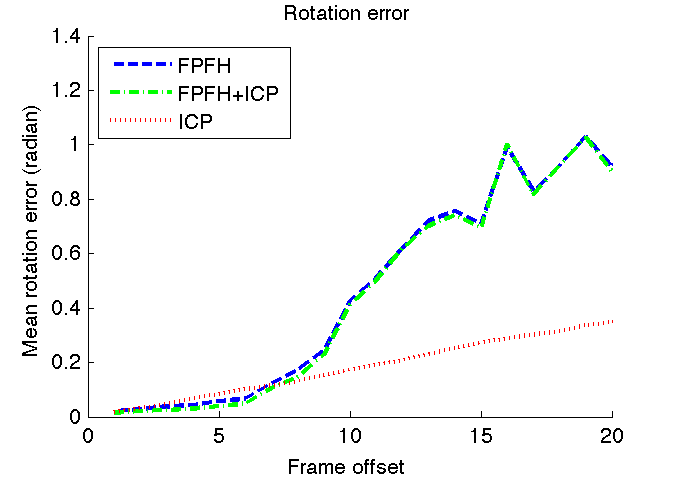
\includegraphics[width=0.49\textwidth]{ims/deskRotationerror.png}
    \caption{The rotation error, i.e. the spherical distance between the estimated rotation and the ground truth rotation, for both datasets.}
    \label{fig:rotation_error}
\end{figure}

Figures ~\ref{fig:rotation_error} and~\ref{fig:translation_error} show that the combination of a feature-based initial alignment with an \ac{ICP} refinement can give the best results. Interestingly, as can be seen in~\ref{fig:rotation_error} using only \ac{FPFH} performs worse than using only \ac{ICP}, but when combined it allows \ac{ICP} to find a better solution. However, when the discrepancy between frames gets larger (more frames are skipped), it seems like the \ac{FPFH} method starts failing and `drags' \ac{ICP} along with it, away from the correct solution. This is easy to see in the right figures, but we found that it also occurred on the other dataset, when skipping more frames than shown here. We think this might be caused by the fact that feature based methods are more likely to produce large transforms; making it likely that they produce large errors. 


\begin{figure}[H]
    \centering
        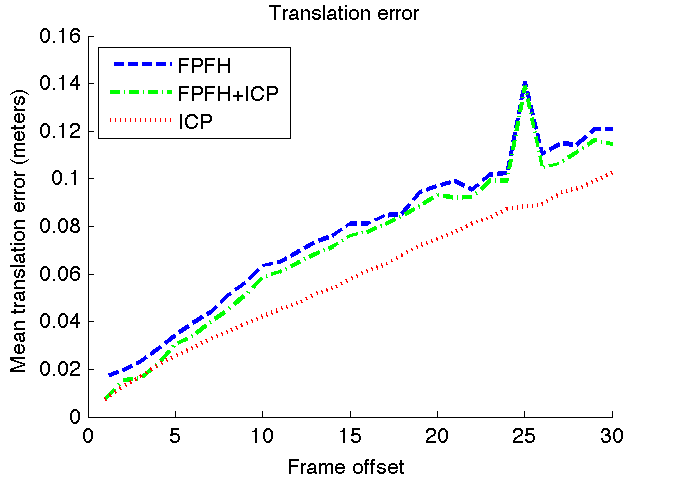
\includegraphics[width=0.49\textwidth]{ims/xyzTranslationerror.png}
        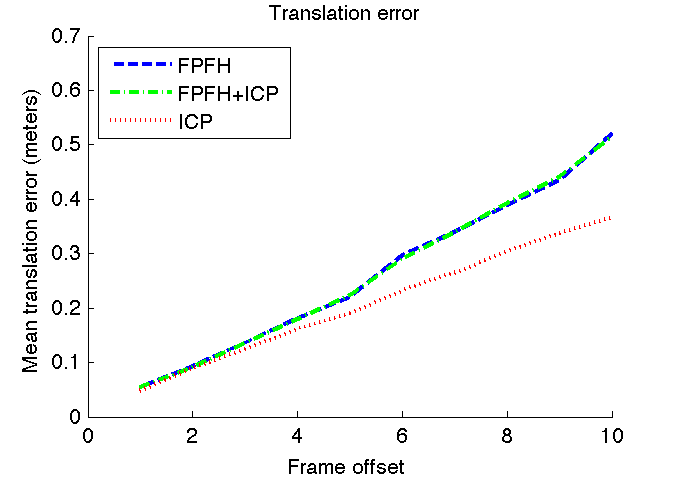
\includegraphics[width=0.49\textwidth]{ims/deskTranslationerror.png}
    \caption{The translation error, i.e. the euclidian distance between the estimated translation and the ground truth translation, for both datasets.}
    \label{fig:translation_error}
\end{figure}


\section{Discussion}

According to Figures~\ref{fig:rotation_magnitude} and~\ref{fig:translation_magnitude} \ac{ICP} underestimates the rotation and translation. The feature-based methods do indeed come up with much larger transformation. The counterintuitive result is that the smaller transformations estimated by \ac{ICP} result in a smaller mean error, even though the ground truth transformation is larger. This seems to indicate that \ac{ICP} moves a small distance in the right direction, whereas the feature-based method performs a larger transformation that does not necessarily move it closer to the true pose. This effect might be because the feature-based method finds the \emph{wrong} feature correspondences when little overlap is available.

We thought that \ac{ICP} would only work with small transformations between frames, and that it's effectiveness would decrease with increasing discrepancy between frames. This seemed to be the case when we did a qualitative analysis of the registration results by viewing the global models. For this reason we thought that using fewer frames to reduce the error buildup would be detrimental to \ac{ICP}'s performance. However, this hypothesis does not seem to be confirmed by our experiments.

The experiments show that there is an optimal selection of frames that yields the lowest error over longer periods. When simply using only every n-th frame, this is still subject to the characteristics of the dataset. It is necessary to balance the performance of single pairs with the performance over a longer time. Using a fixed and constant portion of the frames is generally a bad idea because most input data will not be homogeneous (i.e. the magnitude of the transformation between each pair of frames will usually vary). Therefore it is necessary to use a \emph{keyframe selection} method, which decides whether or not to discard each frame based on the aforementioned factors.

In summation, it seems like it is indeed necessary to use a feature based initial alignment before refining the registration, for best results. \ac{ICP} only performs well when using very similar frames, but this will cause a large build-up of error. In all of the papers where \ac{ICP} was used without initial alignment, some extra techniques were used to prevent this.


\bibliography{../../literature/refs}{}
\bibliographystyle{apalike}

\end{document}
